\documentclass{article}

\usepackage{graphicx}
\usepackage{tikz}
\usepackage{tikzsymbols}
\usetikzlibrary{calc,patterns,shapes.geometric}
\pagestyle{empty}
\usepackage[margin=0pt]{geometry}
\geometry{papersize={14in,12in}}

\def\centerarc[#1](#2)(#3:#4:#5){\draw[#1] ($(#2)+({#5*cos(#3)},{#5*sin(#3)})$) arc (#3:#4:#5);}

\begin{document}
	\begin{figure}
		\centering
		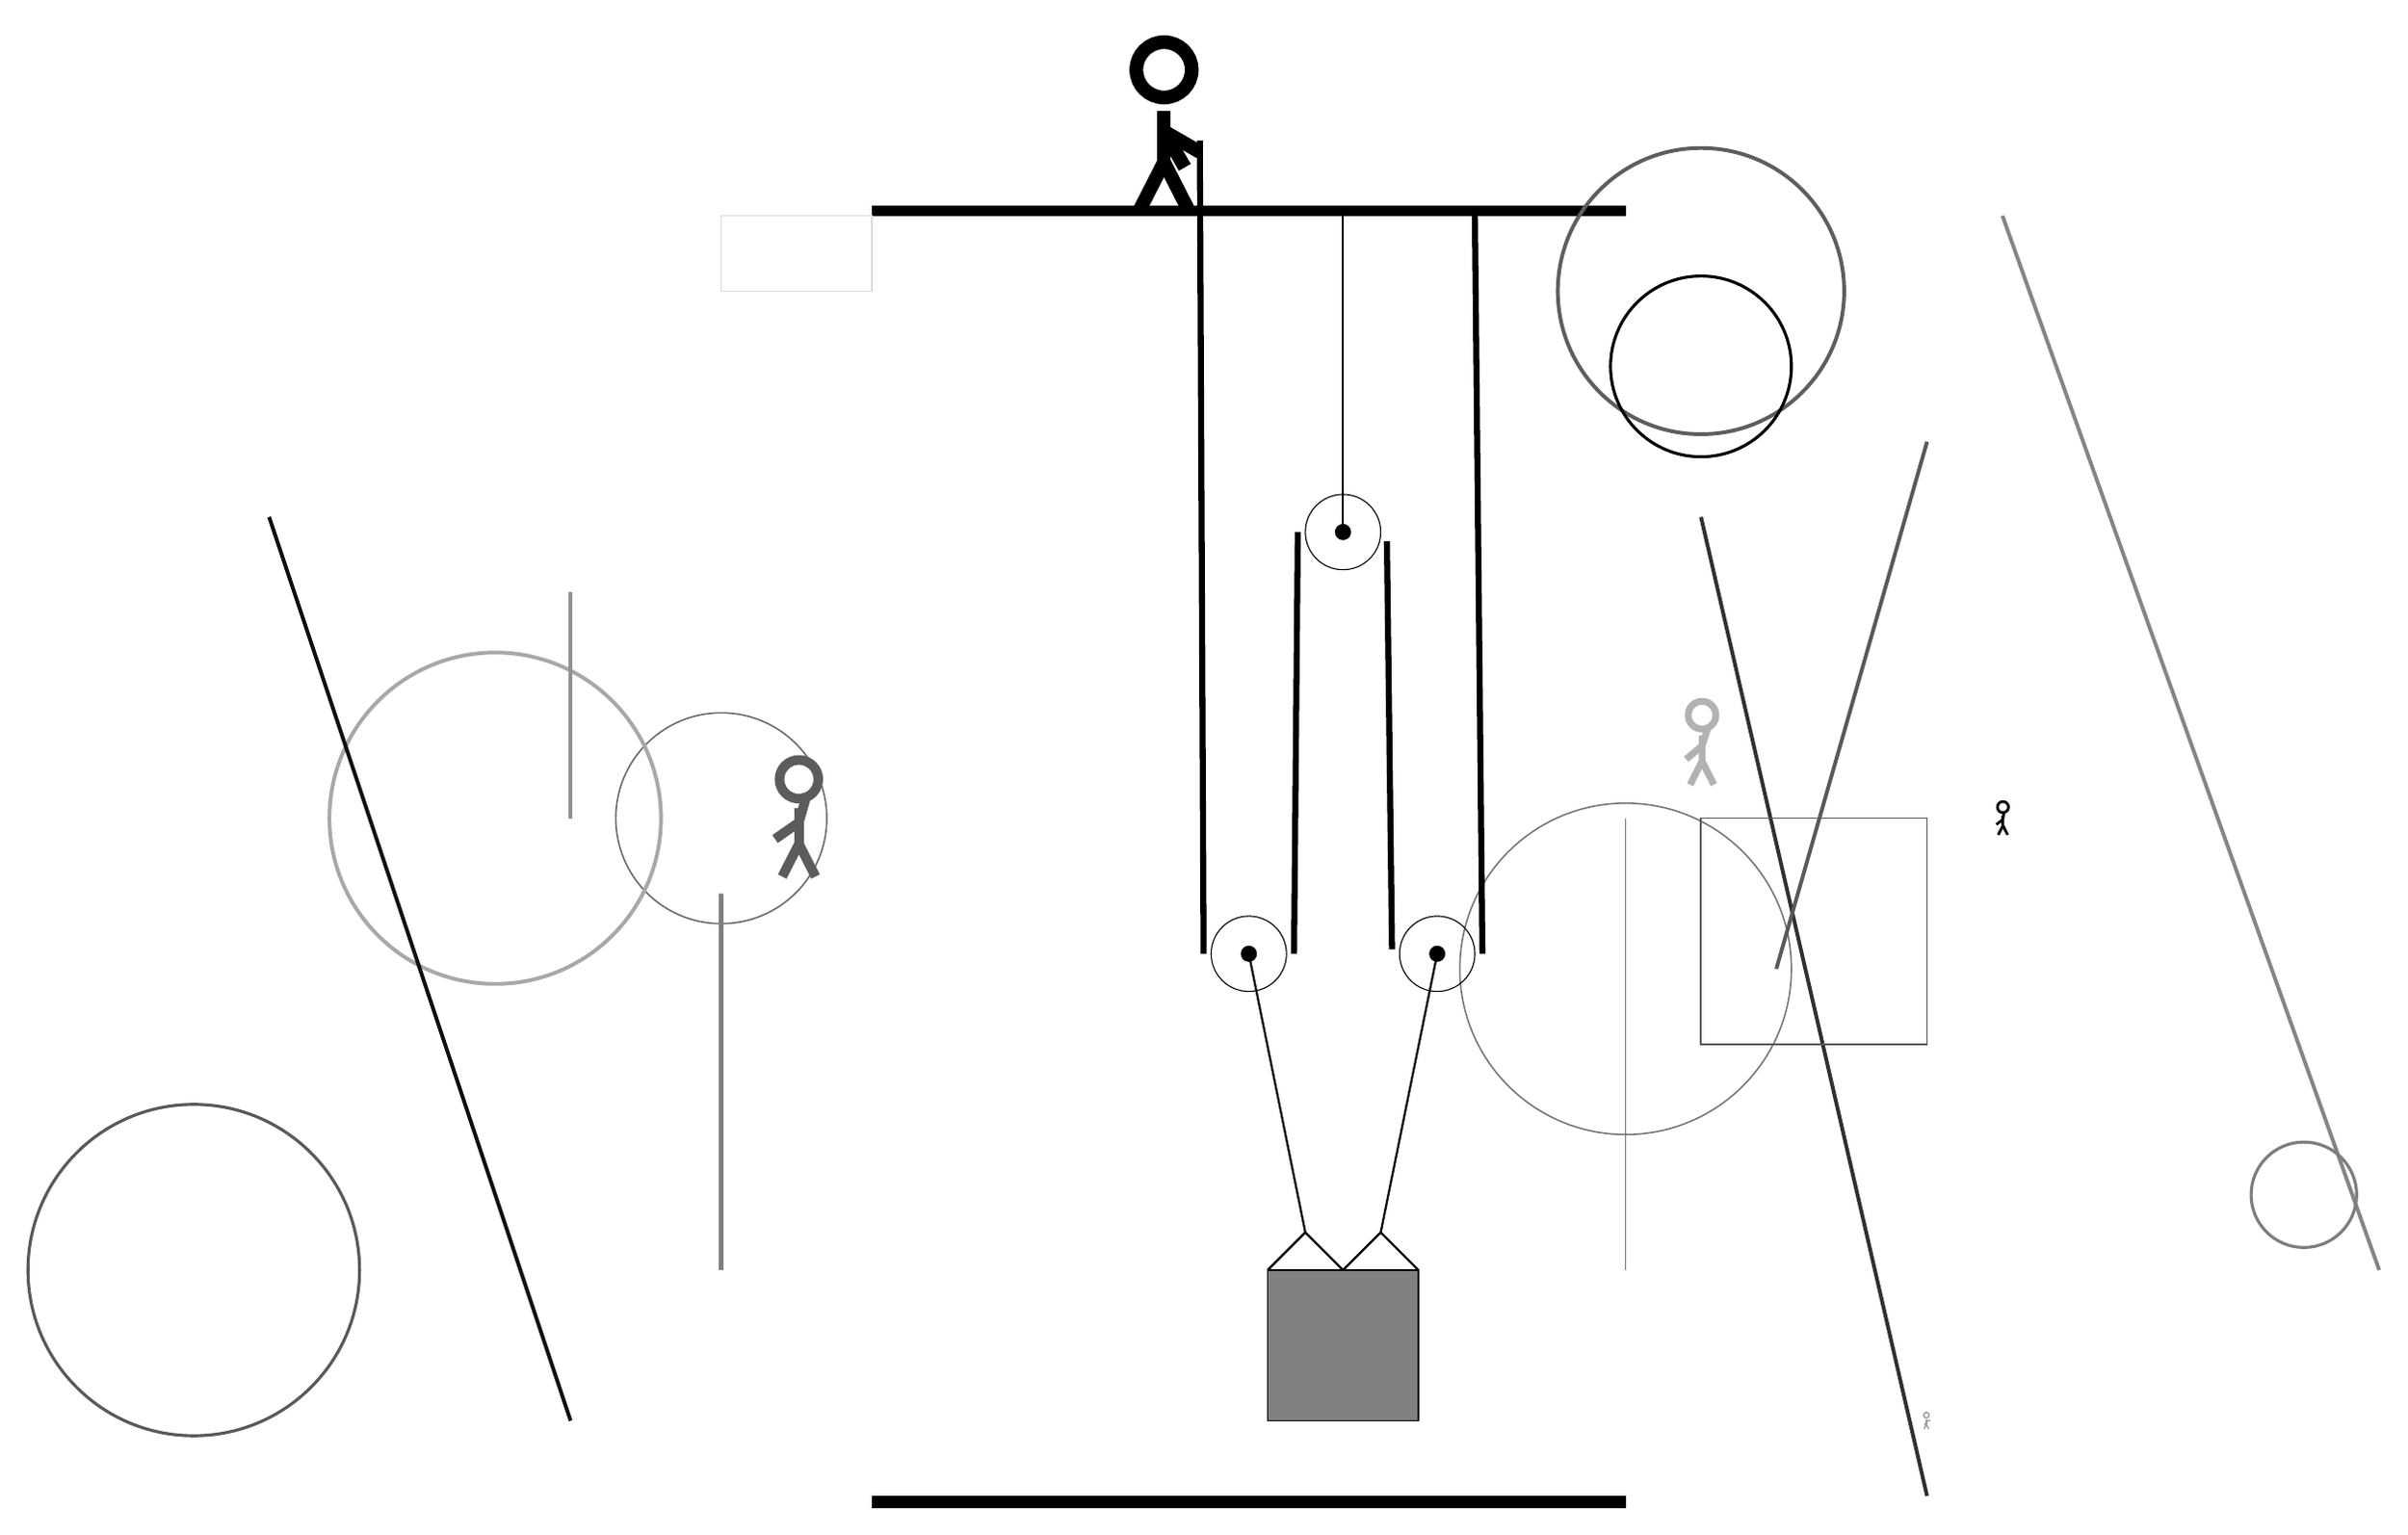
\begin{tikzpicture}
			%%%%% START %%%%%
			
			\draw[fill=black] (-4, 14) rectangle (6, 14.125);
			
			\draw (1, 4.2) circle (0.5);
			\draw[fill=black] (1, 4.2) circle (0.1);
			
			\draw [line width=0.4mm, color=black!65](-13, 0) circle (2.2);
			
			\draw[line width=0.2mm, color=black!53] (6, 6) rectangle (6, 0);
			\draw[line width=0.5mm, color=black!48](11, 14) -- (16, 0);
			\draw[line width=0.2mm, color=black!14] (-6, 13) rectangle (-4, 14);
			\draw [line width=0.5mm, color=black!63](7, 13) circle (1.9);
			\draw [line width=0.4mm, color=black!51](15, 1) circle (0.7);
			\draw [line width=0.2mm, color=black!59](-6, 6) circle (1.4);
			
			\draw[line width=0.5mm, color=black!81](10, -3) -- (7, 10);
			\node[line width=0.7mm, color=black!30] at (7, 7) {\Strichmaxerl[5][40][72]};
			
			\node[line width=0.6mm, color=black!38] at (10, -2) {\Strichmaxerl[1][66][14]};
			\draw [line width=0.2mm, color=black!45](7, 6) circle (0.0);
			
			\draw [line width=0.2mm, color=black!54](6, 4) circle (2.2);
			\draw[line width=0.2mm, color=black!65] (7, 6) rectangle (10, 3);
			
			\draw [line width=0.5mm, color=black!34](-9, 6) circle (2.2);
			\draw[line width=0.5mm, color=black!94](-8, -2) -- (-12, 10);
			\draw[line width=0.5mm, color=black!43](-8, 9) -- (-8, 6);
			\node[line width=0.2mm, color=black!64] at (-5, 6) {\Strichmaxerl[7][35][74]};
			\draw [line width=0.4mm, color=black!98](7, 12) circle (1.2);
			\draw[line width=0.5mm, color=black!65](8, 4) -- (10, 11);
			\draw[line width=0.6mm, color=black!50] (-6, 5) rectangle (-6, 0);
			\node[line width=0.2mm, color=black!96] at (11, 6) {\Strichmaxerl[2][38][82]};
			
			
			\draw (2.25, 9.8) circle (0.5);
			\draw[fill=black] (2.25, 9.8) circle (0.1);
			\draw[thick] (2.25, 9.8) -- (2.25, 14);
			
			\draw (3.5, 4.2) circle (0.5);
			\draw[fill=black] (3.5, 4.2) circle (0.1);
			
			\draw[thick] (3.5, 4.2) -- (2.75, 0.5);
			\draw[thick] (1, 4.2) -- (1.75, 0.5);
			\draw[thick]  (1.25, 0) -- (1.75, 0.5) -- (2.25, 0);
			\draw[thick]  (2.25, 0) -- (2.75, 0.5) -- (3.25, 0);
			\draw[fill=black!50] (1.25, 0) rectangle (3.25, -2);
			
			\draw[line width=0.8mm] (0.35, 15) --  (0.4, 4.2);
			\centerarc[line width=0.8mm](1, 4.2)(180:360:0.6);
			\draw[line width=0.8mm] (1.6, 4.2) -- (1.65, 9.8);
			\centerarc[line width=0.8mm](2.25, 9.8)(-20:180:0.6);
			\draw[line width=0.8mm](2.832, 9.68) -- (2.9, 4.26);
			\centerarc[line width=0.8mm](3.5, 4.2)(160:360:0.6);
			\draw[line width=0.8mm](4.1, 4.2) -- (4.0, 14);
			
			\node at (-0.07, 15.2) {\Strichmaxerl[10][120][-30]};
			
			\draw[fill=black] (-4, -3) rectangle (6, -3.15);
			
			%%%%% END %%%%%
		\end{tikzpicture}
	\end{figure}	
\end{document}